\documentclass[10pt,twocolumn,letterpaper]{article}

\usepackage{royer_style}
\usepackage[english]{babel}
\usepackage{orcidlink}
\usepackage{multirow}
\usepackage{soul}
\usepackage{enumitem}
\usepackage{booktabs}
\usepackage{ragged2e}
\usepackage{float}
\usepackage{makecell}

% Supplementary Figures
\newfloat{suppfigure}{tbp}{los}
\floatname{suppfigure}{Supplementary Figure}
\renewcommand{\thesuppfigure}{S\arabic{suppfigure}}

% Supplementary Documents
\newfloat{suppdoc}{tbp}{lod}
\floatname{suppdoc}{Supplementary Document}
\renewcommand{\thesuppdoc}{S\arabic{suppdoc}}

% Custom commands
\newcommand{\luxar}{\textsc{Luxar}\xspace}

\title{Luxar: Gaussian splatting and interactive web visualization for multidimensional scientific data}
\author{
    Lo\"ic A. Royer\ts{1}\orcidlink{0000-0002-9991-9724}
}
\affiliation{
\ts{1} Chan Zuckerberg Biohub, San Francisco, United States \\
}
\email{loic.royer@czbiohub.org}

\begin{document}

\twocolumn[
    \maketitle
    \abstract{Sharing and interactively exploring multidimensional scientific data remains a persistent challenge: raw datasets are too large to transfer casually, desktop viewers require local installation, and existing web viewers demand multi-resolution pyramid preprocessing and infrastructure expertise.
    Here we introduce \luxar, an open-source, Python-first system in which a few lines of code compile arbitrary-dimensional data---points, lines, and Gaussian splats---into compact, spatially indexed archives that are served to a browser-based viewer with HDR rendering, progressive streaming, and native $n$-dimensional navigation.
    No web development or server expertise is required.
    We demonstrate \luxar across domains including microscopy, single-cell genomics, and astronomy, and focus on a new capability: fitting microscopy volumes to Gaussian splats---compact, continuous, GPU-renderable primitives that exploit the sparsity of fluorescence data.
    Systematic evaluation on 12~microscopy datasets achieves 13--313$\times$ compression at 25--43~dB PSNR---a 100-million-voxel light-sheet volume shrinks from 400~MB to 1.3~MB while preserving structural fidelity. Blind-spot cross-validation provides a principled criterion for determining when the model has captured all recoverable signal, separating structural information from noise.
    Tiled fitting with cosine apodization removes the GPU memory ceiling.
    \luxar makes volumetric scientific data as easy to share and explore as a web link.}
]

%% ========== INTRODUCTION ==========
\section*{Introduction}

Modern scientific instruments generate multidimensional data at a pace that far outstrips our ability to share and explore it.
A single light-sheet microscope run produces hundreds of gigabytes\cite{keller2008reconstruction,power2017guide}; a single-cell atlas\cite{regev2017humancellatlas} contains millions of cells embedded in high-dimensional spaces; a sky survey such as Gaia\cite{gaiacollaboration2023gaia} catalogs billions of sources with dozens of attributes per object.
Yet the dominant mode of dissemination remains downloading raw files---or, more commonly, inspecting static projections that discard the very dimensionality that motivated the measurement.

Interactive exploration fares no better.
Desktop tools such as napari\cite{sofroniew2022napari}, Fiji\cite{schindelin2012fiji}, Vaa3D\cite{peng2014vaa3d}, and BigDataViewer\cite{pietzsch2015bigdataviewer} provide powerful visualization but require local installation and data download.
Web-based viewers like Neuroglancer\cite{maitinshepard2021neuroglancer} stream voxel data over HTTP but remain limited to axis-aligned slicing and require multi-resolution pyramid preprocessing.
Neither paradigm is designed for the full diversity of scientific data: volumetric microscopy, point-cloud embeddings, polyline trajectories, and higher-dimensional datasets all require different tools, formats, and expertise.

Here we present \luxar (Fig.~\ref{fig:overview}), an open-source system that bridges the gap between data generation in Python and interactive exploration in a web browser.
\luxar supports three first-class geometry types---\textbf{points}, \textbf{lines}, and \textbf{Gaussian splats}---within a hierarchical scene graph that handles arbitrary dimensions, physical units, and per-dimension transforms.
Scientists work entirely in Python and NumPy: a handful of lines compiles data into a chunked Zarr\cite{miles2023zarr} archive with spatial indexing, which is then streamed to a WebGL viewer with HDR rendering, progressive loading, and native $n$-dimensional navigation (Fig.~\ref{fig:overview}a,b).
No knowledge of TypeScript, WebGL, or web development is required; the viewer opens in any modern browser via \texttt{luxar serve data.zarr --viewer}.

This Python-first, compile-then-view architecture enables applications across domains: protein embeddings as color-coded point clouds, cell tracking as splats-plus-polylines, single-cell atlases with categorical dimension navigation, and volumetric microscopy rendered as Gaussian splats (Fig.~\ref{fig:overview}c).
In this paper, we focus on the last of these---Gaussian splatting for microscopy volumes---which represents the most technically novel contribution.

Fluorescence microscopy data is inherently sparse: signal is concentrated in structures---nuclei, membranes, filaments---while the vast majority of voxels are background.
Gaussian splatting\cite{kerbl2023gaussian,yun2024gsplat}, originally developed for real-time novel-view synthesis as an alternative to neural radiance fields\cite{mildenhall2021nerf}, represents a volume as a mixture of oriented, anisotropic Gaussian primitives, placing representational capacity only where signal exists.
The resulting representation is continuous, compact, and directly GPU-renderable---properties that align precisely with the needs of microscopy data dissemination.

We adapt Gaussian splatting for microscopy with a purpose-built optimization pipeline featuring per-splat Adam optimization with dynamic topology and Cholesky-parameterized covariance.
We validate the approach on 12~datasets spanning confocal, spinning-disk, and light-sheet modalities, and show via blind-spot cross-validation\cite{batson2019noise2self} that the noise level sets an upper bound on useful model complexity---providing a principled criterion for separating signal from noise.
Tiled fitting with cosine apodization removes the GPU memory ceiling, enabling reconstruction of arbitrarily large volumes via embarrassingly parallel computation.


%% ========== RESULTS ==========
\section*{Results}

\paragraph{The \luxar system.}
\luxar is designed around a simple principle: scientists should describe their data in Python and explore it in a browser, without requiring web development expertise.
The core API exposes three geometry types---\texttt{Points} (positions, colors, radii), \texttt{Lines} (vertices, widths, colors), and \texttt{GSplats} (centers, amplitudes, Cholesky factors)---organized in a hierarchical scene graph with groups, transforms, and $n$-dimensional coordinate systems (Fig.~\ref{fig:overview}a).

A \texttt{LuxarZarrCompiler} context manager writes data progressively to Zarr, enabling datasets far exceeding RAM to be compiled on a laptop.
Each geometry node is spatially indexed via Morton (Z-order) curves, chunked, and compressed with Blosc/zstd.
The compiled archive is served over HTTP and rendered by a WebGL viewer with a three-level cache (persistent browser storage, compressed RAM, decompressed GPU buffers), 16-bit HDR tone mapping, and configurable anti-aliasing and post-processing.

For $n$-dimensional datasets, displayed spatial dimensions are navigated by orbiting and zooming; non-displayed dimensions (time, channel, experimental condition) are navigated via continuous sliders or categorical toggles.
Gaussian splats and points are treated as hyperspheres in $n$D; visibility is determined by hypersphere--hyperplane intersection, computed via an inverse-query approach in O(1) per dimension.

\paragraph{Fitting microscopy volumes to Gaussian splats.}
\luxar decomposes a microscopy volume $V: \mathbb{R}^D \to \mathbb{R}_{\geq 0}$ into a mixture of $K$ anisotropic Gaussians:
\begin{equation}
\hat{V}(\mathbf{x}) = \sum_{k=1}^{K} a_k \exp\!\left(-\tfrac{1}{2}\left\|\mathbf{L}_k^{-1}(\mathbf{x} - \boldsymbol{\mu}_k)\right\|^2\right)
\label{eq:gsplat}
\end{equation}
where $\boldsymbol{\mu}_k$ is the position, $a_k > 0$ the amplitude, and $\mathbf{L}_k$ the Cholesky factor of the covariance ($\boldsymbol{\Sigma}_k = \mathbf{L}_k \mathbf{L}_k^\top$), ensuring positive-definiteness by construction.
Parameters are optimized via a per-splat Adam optimizer\cite{kingma2015adam} with individual momentum states, enabling dynamic operations---relocation, pruning, and seeding---without disrupting existing primitives.
The reconstruction loss is L1 with regularization on splat amplitudes and extents (see Methods).
Initial positions are determined by GPU-accelerated edge detection (see Methods).

\paragraph{Reconstruction quality across microscopy modalities.}
We evaluated reconstruction across 12~datasets spanning spinning-disk confocal (OpenCell\cite{cho2022opencell}), standard confocal (kidney tissue, intestinal organoid, \emph{C.~elegans} embryo), and light-sheet (Tribolium embryo) modalities, with volumes from 4~to 100~million voxels (Table~\ref{tab:summary}; 7 representative datasets shown, all 12 in Supplementary Document~2).

All datasets exhibit a log-linear rate-distortion relationship (Fig.~\ref{fig:ratedistortion}a).
The Tribolium light-sheet volume ($\sigma = 0.0009$) plateaus at 32K~splats with 42.6~dB PSNR and 313$\times$ compression (Fig.~\ref{fig:visual}i--l).
Kidney tissue achieves 33.7~dB at 32K~splats and continues to 37.3~dB at 512K (Fig.~\ref{fig:visual}a--d).
SSIM follows a similar pattern (Fig.~\ref{fig:ratedistortion}b).
At 32K~splats, compression ratios range from 13$\times$ to 313$\times$ with 25--43~dB PSNR (Fig.~\ref{fig:ratedistortion}c, Table~\ref{tab:summary}), and fitting completes in 10--60~seconds on a consumer GPU.

\paragraph{Cross-validation identifies the boundary between signal and noise.}
The number of splats needed to represent a volume is primarily determined by its information content---the structural complexity of the biological signal.
However, adding splats beyond what the signal requires causes the model to memorize noise.
We used blind-spot cross-validation---masking 5\% of voxels and replacing them with donut-median neighborhood values\cite{batson2019noise2self}, then evaluating held-out reconstruction---to detect this transition.

The held-out PSNR peaks and then declines for 6 of 7~core datasets (Fig.~\ref{fig:ratedistortion}d, Supplementary Document~2).
For kidney DAPI ($\sigma = 0.009$), the train--held-out gap widens to 5.9~dB at 512K~splats, indicating that splats beyond the 63K optimum are fitting noise rather than structure.
Across datasets, the noise level constrains useful model capacity (Fig.~\ref{fig:ratedistortion}f): the held-out peak provides a per-dataset stopping criterion, with noisier datasets generally reaching their ceiling at fewer splats, though structural complexity also plays a role.
This provides a practical recipe: fit at increasing capacity, stop at the held-out peak.

The sole exception is the Tribolium light-sheet volume, where train and held-out curves are virtually identical (Fig.~\ref{fig:ratedistortion}e).
This dataset was produced by multi-view deconvolution\cite{preibisch2014efficient}, a process that introduces spatial correlations in the residual noise, violating the pixel-independence assumption underlying the blind-spot framework.
Consequently, the blind-spot validation cannot distinguish signal from noise in this case---the model appears signal-limited at all tested capacities.
Nevertheless, the reconstruction quality itself plateaus (42.6~dB at 32K splats), providing a practical stopping criterion: additional splats yield negligible improvement, regardless of whether the ceiling reflects noise or signal exhaustion.

\paragraph{Tiled fitting for scalability.}
For volumes exceeding GPU memory, \luxar partitions the volume into overlapping tiles, each fitted independently, and concatenates the results.
Cosine (Hann) apodization windows ensure a partition of unity at tile boundaries---adjacent windows sum to exactly 1.0---eliminating visible seams.
Tiles are embarrassingly parallel: they distribute across GPUs, cluster nodes, or Slurm array jobs---a 2048$^3$ volume that would exceed consumer GPU memory (e.g., NVIDIA RTX~3090, 24~GB) can be processed as overlapping 256$^3$ tiles.
The \luxar batch system handles OME-Zarr\cite{moore2021ome} 5D layouts (time, channel, Z, Y, X) with automatic fan-in merging.

\paragraph{Viewer performance.}
In benchmarks on an NVIDIA RTX~3070, the web viewer maintains 60~FPS for scenes up to 500,000 elements, with uncapped GPU throughput exceeding 2,000~renders/second for 100K GSplats during interactive camera orbit (Supplementary Table~1).
GSplat scenes load in under one second; larger point-cloud datasets (millions of elements) render at full frame rate once loaded, though initial transfer time scales with dataset size even with progressive streaming.


%% ========== DISCUSSION ==========
\section*{Discussion}

\luxar addresses a gap that has widened with each generation of scientific instruments: the data we can acquire has outgrown the tools we have to share and explore it.
By separating data \emph{compilation} (in Python, where scientists already work) from \emph{rendering} (in a web browser, where no installation is needed), \luxar makes multidimensional scientific data as easy to share as a web link.

The Python-first design is deliberate.
The bioimaging community, and scientific computing more broadly, has converged on Python as the common language\cite{sofroniew2022napari,vanderWalt2014scikit}---from acquisition control and analysis pipelines to machine learning frameworks.
\luxar meets scientists where they are: a few lines of NumPy and \luxar produce an interactive, streamable visualization without requiring web development skills.
This stands in contrast to existing approaches that either require desktop software (napari\cite{sofroniew2022napari}, Fiji\cite{schindelin2012fiji}) or web-development expertise (custom Neuroglancer\cite{maitinshepard2021neuroglancer} deployments).
Compared with these tools, \luxar occupies a distinct niche: it requires neither local installation nor multi-resolution pyramid preprocessing, supports mixed geometry types (not just voxels), and achieves 10--300$\times$ compression that makes data transfer practical even over modest bandwidth (Supplementary Fig.~3).
Rendering performance is sufficient for interactive exploration of all tested scene sizes (Supplementary Table~1).

The Gaussian splatting contribution extends this accessibility to volumetric microscopy.
The core insight is that fluorescence data is sparse, and Gaussian splats exploit this sparsity by placing representational capacity only where signal exists.
Our cross-validation analysis provides a principled way to determine how much representational capacity a given dataset warrants: the information content of the volume drives the splat count upward, while the noise level caps it.
At the optimal count, splats capture the recoverable signal while naturally discarding noise---without an explicit denoising step.
For light-sheet data, the representation is extraordinarily compact (313$\times$ compression); for noisier confocal data, a lower splat count yields higher-fidelity reconstructions than blindly adding more.
When compared against H.265 video compression using a blind-spot held-out framework that measures true signal recovery, Gaussian splats achieve up to 3~dB higher held-out PSNR on noisy confocal data (Supplementary Fig.~3).
The splat representation is additionally \emph{directly renderable} without decompression.
We also find that single-pass fitting with conservative culling outperforms progressive multi-pass approaches at a fixed splat budget for 8 of 12~datasets, while 2-pass progressive fitting yields +0.9 to +1.6~dB gains for clean, well-structured volumes---and is 1.2--4.4$\times$ faster (Supplementary Fig.~4; Supplementary Document~3).

While this paper focuses on microscopy, \luxar is domain-agnostic.
The same system visualizes millions of stars from astronomical surveys\cite{gaiacollaboration2023gaia}, hundreds of thousands of cells from single-cell atlases\cite{tabula2022tabula} (Tabula Sapiens), protein embeddings, super-resolution localizations, and cell tracking trajectories mixing Gaussian splats with polyline overlays---all with native $n$-dimensional navigation (Fig.~\ref{fig:overview}c).
We envision \luxar as infrastructure: a common layer between Python-based data generation and interactive, web-based exploration, applicable wherever scientists produce multidimensional data and need to share it.

Limitations include the inherent approximation of Gaussian splats, which can blur thin filamentous structures (e.g., individual microtubules) where the Gaussian shape is a poor local fit; coordination overhead for very large tiled fits on HPC systems (automatic volume partitioning is not yet supported); the absence of quantitative intensity analysis (the representation targets visualization and sharing, not downstream tasks such as segmentation or tracking); and a light-sheet evaluation limited to a single dataset, though we expect broader light-sheet coverage in future work.
The cross-validation model-selection procedure requires fitting at multiple splat counts, though each fit takes only 10--60~seconds, making a full sweep practical.

\luxar is open source and installable via \texttt{pip install luxar}.
Code, documentation, and live demos are available at \url{https://github.com/royerlab/luxar}.


%% ========== FIGURES ==========

\begin{figure*}[t]
    \centering
    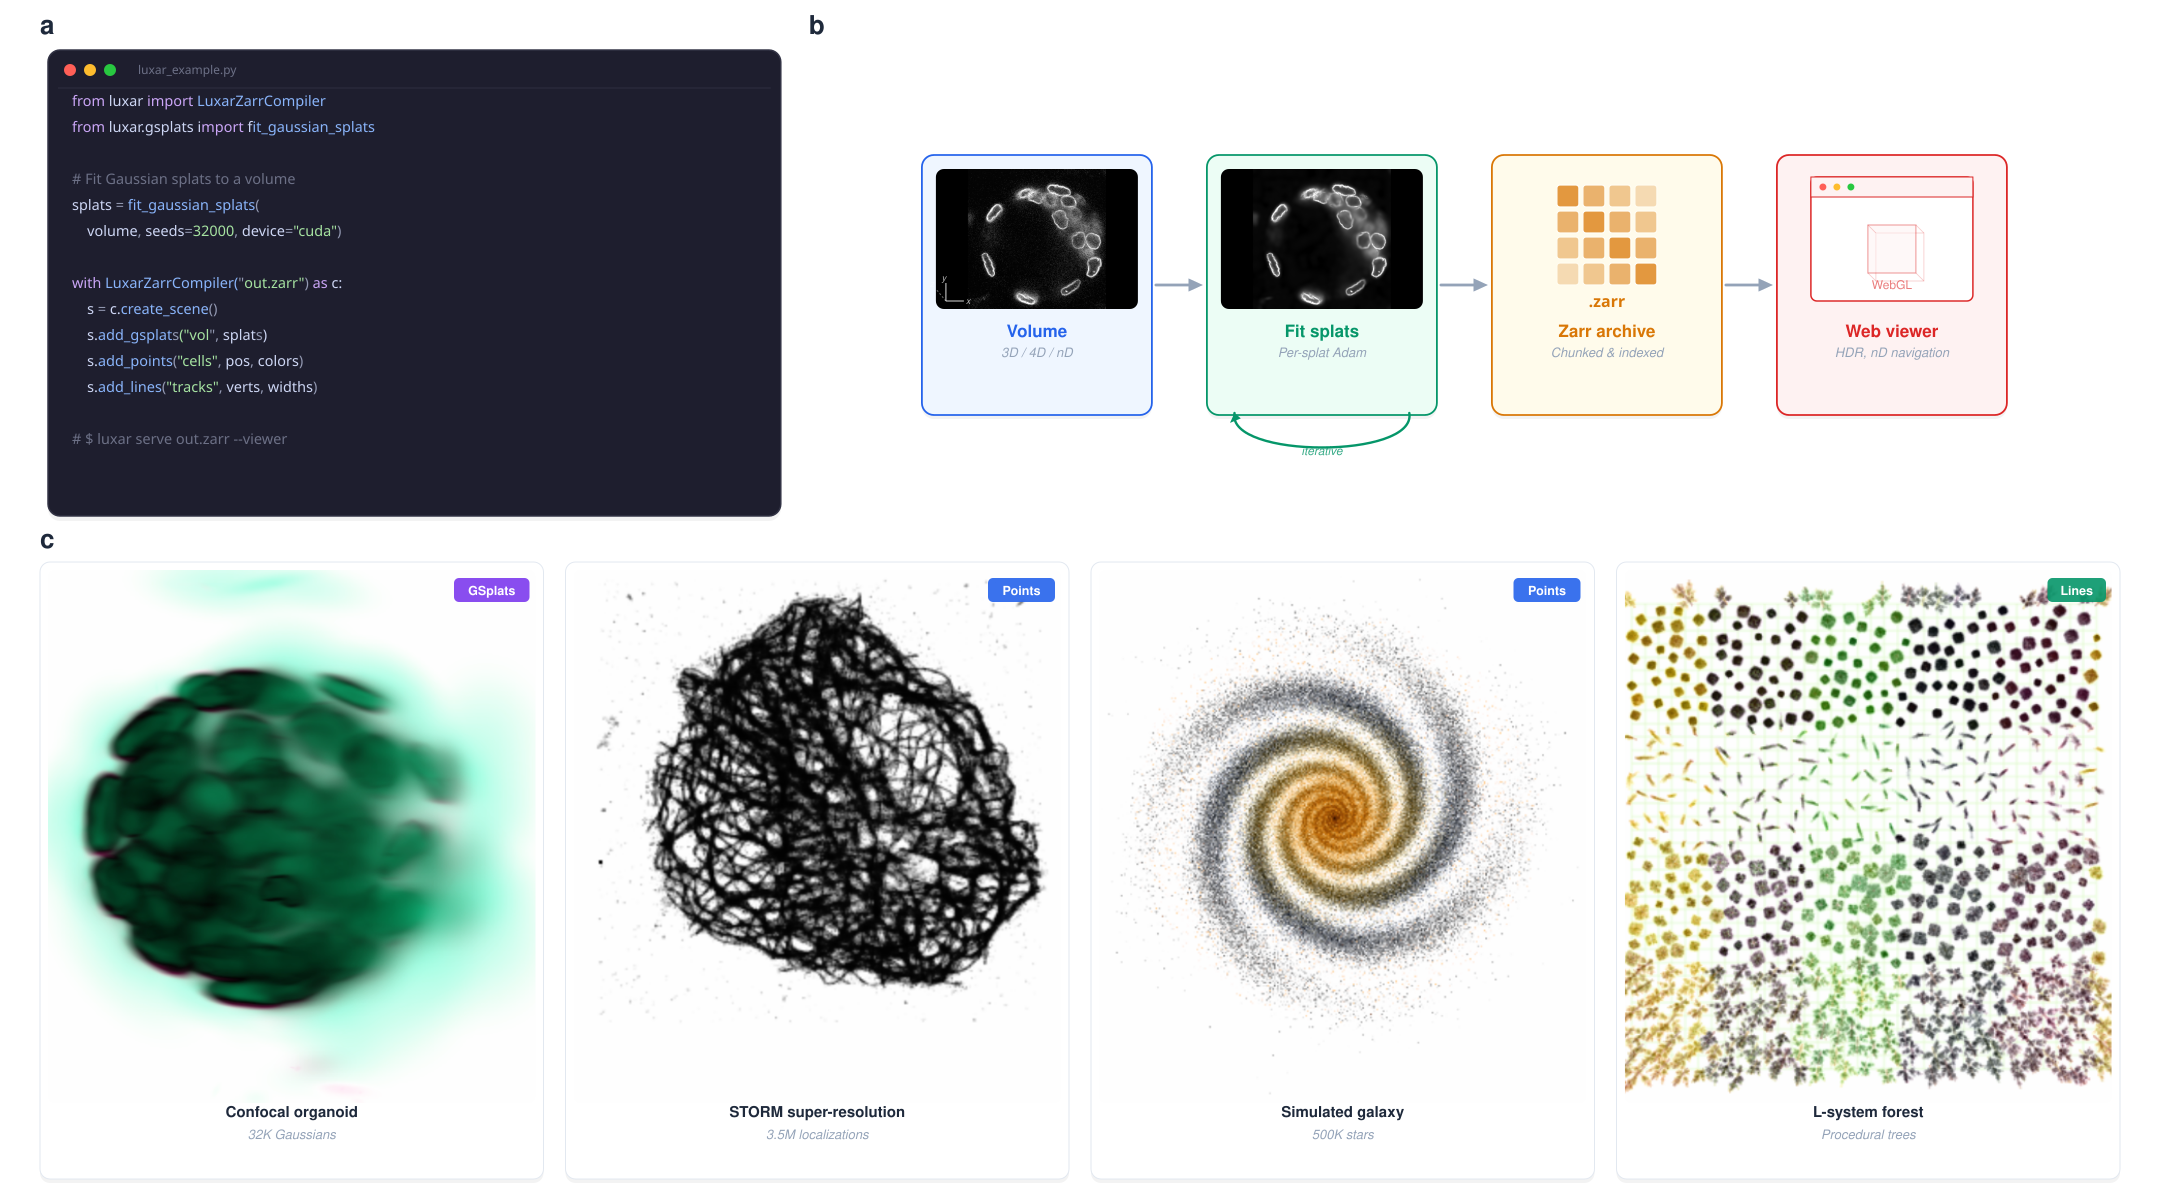
\includegraphics[width=\textwidth]{figs/overview/overview.pdf}
    \vspace{-0.5em}
    \caption{\textbf{The \luxar system: from Python to interactive web visualization.}
    \textbf{a,} Scientists work entirely in Python: a few lines of code compile data (points, lines, or Gaussian splats) into a spatially indexed Zarr archive with $n$-dimensional coordinates.
    \textbf{b,} Data flows from NumPy arrays through a hierarchical scene graph to a chunked archive, served over HTTP to a browser-based WebGL viewer with HDR rendering, progressive streaming, and $n$-dimensional navigation.
    \textbf{c,} \luxar viewer screenshots showing application breadth across geometry types and scientific domains: Gaussian splats for a confocal organoid, points for 3.5M STORM super-resolution localizations, points for a 500K-star simulated galaxy, and lines for procedurally generated L-system trees.
    No web development required---the viewer opens in any browser.}
    \label{fig:overview}
\end{figure*}

\begin{figure*}[t]
    \centering
    \includegraphics[width=\textwidth]{figs/visual_comparison/visual_comparison.pdf}
    \caption{\textbf{Visual quality of Gaussian splat reconstructions across modalities.}
    Representative slices at increasing splat counts.
    \textbf{a--d,} Mouse kidney\cite{vanderWalt2014scikit} (confocal, DAPI): 128K splats recover fine nuclear morphology at 3$\times$ compression.
    \textbf{e--h,} 3D cell culture\cite{blin2019nessys} (confocal, mouse ESC acini): lumenal structure and cell boundaries faithfully reconstructed.
    \textbf{i--l,} Tribolium embryo\cite{preibisch2014efficient} (light-sheet): 4K splats capture the full morphology at 2{,}512$\times$ compression ($\sigma = 0.0009$).
    White annotations: PSNR and compression ratio. Scale bars in original panels.}
    \label{fig:visual}
\end{figure*}

\begin{figure*}[t]
    \centering
    \includegraphics[width=\textwidth]{figs/quantitative_analysis/quantitative_analysis.pdf}
    \caption{\textbf{Quantitative analysis and noise-aware model selection.}
    \emph{Top row:} rate-distortion analysis across 7~representative datasets (of 12 total).
    \textbf{a,} PSNR vs.\ splat count. All datasets show log-linear improvement.
    \textbf{b,} SSIM vs.\ splat count.
    \textbf{c,} PSNR vs.\ compression ratio (higher compression to the left).
    \emph{Bottom row:} Blind-spot cross-validation.
    \textbf{d,} Kidney DAPI (confocal): held-out PSNR peaks at 63K splats (star) then declines---a 5.9~dB overfitting gap at 512K.
    \textbf{e,} Tribolium (light-sheet): no overfitting; train and held-out curves overlap.
    \textbf{f,} Optimal splat count (held-out peak) varies with noise level and structural complexity: noisier data generally saturates at fewer splats. Tribolium excluded (no held-out peak; see text).}
    \label{fig:ratedistortion}
\end{figure*}

%% ========== TABLE ==========
\begin{table*}[t]
\centering
\small
\caption{\textbf{Gaussian splat reconstruction quality across microscopy modalities.} PSNR, SSIM, and compression ratio (CR) at 32K splats; best PSNR at 512K splats; estimated noise floor; and cross-validation-optimal splat count. Volumes normalized to $[0, 1]$.}
\label{tab:summary}
\begin{tabular}{@{}llccccccc@{}}
\toprule
Dataset & Modality & Shape & \makecell{PSNR\\@32K} & \makecell{SSIM\\@32K} & \makecell{CR\\@32K} & \makecell{Best\\PSNR} & \makecell{Noise\\floor} & \makecell{CV\\optimal} \\
\midrule
  Kidney DAPI & Confocal & \footnotesize{16$\times$512$\times$512} & 33.7 & 0.962 & 13$\times$ & 37.3 & 41.3 & 63K \\
  Kidney actin & Confocal & \footnotesize{16$\times$512$\times$512} & 30.5 & 0.895 & 13$\times$ & 37.1 & 43.5 & 124K \\
  MAP4 (Hoechst) & Spinning-disk & \footnotesize{51$\times$600$\times$600} & 28.3 & 0.675 & 57$\times$ & 29.9 & 32.6 & 32K \\
  MAP4 (GFP) & Spinning-disk & \footnotesize{51$\times$600$\times$600} & 25.1 & 0.619 & 57$\times$ & 27.6 & 30.4 & 62K \\
  Organoid & Confocal & \footnotesize{236$\times$275$\times$271} & 39.0 & 0.933 & 62$\times$ & 41.0 & 54.4 & 28K \\
  C. elegans & Confocal & \footnotesize{41$\times$512$\times$512} & 39.3 & 0.893 & 34$\times$ & 40.4 & 40.7 & 16K \\
  Tribolium & Light-sheet & \footnotesize{991$\times$104$\times$965} & 42.6 & 0.993 & 313$\times$ & 42.7 & 61.0 & 32K \\
\bottomrule
\end{tabular}
\end{table*}



%% ========== METHODS ==========
%% ========== METHODS ==========
\section*{Methods}

\paragraph{Gaussian splat model.}
Each splat $k$ is parameterized by a center $\boldsymbol{\mu}_k \in \mathbb{R}^D$, a positive amplitude $a_k$ (via softplus activation), and a lower-triangular Cholesky factor $\mathbf{L}_k \in \mathbb{R}^{D \times D}$.
An optional sharpness exponent $s_k$ (via softplus, clamped to $[1.5, 4.0]$) generalizes the Gaussian shape; all results in this paper use the standard Gaussian ($s_k = 2$).
The model prediction at voxel $\mathbf{x}$ is
$\hat{V}(\mathbf{x}) = \sum_{k} a_k \exp\!\left(-\frac{1}{2}\|\mathbf{L}_k^{-1}(\mathbf{x} - \boldsymbol{\mu}_k)\|^{2}\right)$.
The Cholesky parameterization stores $D(D{+}1)/2$ elements per splat (6 for 3D) and guarantees positive-definite covariance by construction.
Amplitudes are clamped to $[0, \infty)$ via softplus with a configurable $\beta$ parameter.

\paragraph{Optimization.}
We use a per-splat Adam optimizer\cite{kingma2015adam} ($\beta_1{=}0.9$, $\beta_2{=}0.999$, $\epsilon{=}10^{-8}$) that maintains individual momentum and variance accumulators for each splat's parameters.
This enables dynamic operations (relocation, pruning, seeding of new splats) without disrupting the optimization state of existing splats.
The base learning rate is $0.01$ with dimensional compensation: for $D$-dimensional data, the effective learning rate is scaled by $D^{0.8} \times P_D / P_2$, where $P_D$ is the number of parameters per splat in $D$ dimensions.

The loss function is:
\begin{equation}
\mathcal{L} = \mathcal{L}_\text{recon} + \lambda_a \|\mathbf{a}\|_1 + \lambda_d \|\text{diag}(\mathbf{L})\|_1 + \lambda_b \mathcal{L}_\text{boundary}
\end{equation}
where $\mathcal{L}_\text{recon}$ is an asymmetric L1 loss that penalizes over-prediction $10\times$ more than under-prediction, $\lambda_a = 10^{-5}$ and $\lambda_d = 10^{-4}$ regularize splat amplitude and extent, and $\mathcal{L}_\text{boundary}$ penalizes splats whose centers fall outside the volume.

\paragraph{Dynamic operations.}
Every 500 iterations, the optimizer performs dynamic topology adjustment: (1) splats with amplitude below a threshold ($10^{-4}$ of the volume maximum) are pruned; (2) residual-guided relocation moves the lowest-amplitude splats to positions of peak reconstruction error; (3) Z-order (Morton code) sorting is applied to improve GPU cache locality.
The relocation step detects under-represented regions by computing $|\hat{V} - V|$, finding local maxima in the residual, and teleporting selected splats to these positions while preserving their momentum states.

\paragraph{Seed generation.}
Initial splat positions are determined by edge-based seeding: Sobel gradients are computed across all dimensions, local peaks in gradient magnitude are detected, and positions are deduplicated with a minimum separation criterion.
The number of seeds requested typically exceeds the final count, as pruning removes low-amplitude splats during optimization.
Seeding supports GPU acceleration (CUDA, MPS) for 10--50$\times$ speedup on large volumes.

\paragraph{Tiled fitting.}
For volumes exceeding GPU memory, \luxar partitions the volume into overlapping tiles on a regular grid with stride $T - L$, where $T$ is the tile size and $L$ is the overlap.
Each tile is fitted independently with the same optimizer configuration.
Splat amplitudes are modulated by a cosine (Hann) window $w(k) = \frac{1}{2}(1 - \cos(\pi k / (L+1)))$ applied along each overlap face, producing a partition-of-unity: adjacent windows sum to 1.0.
Boundary faces retain unit weight.
The constraint $L \leq T/2$ prevents triple overlap.
After fitting, tiles are concatenated into a single splat dataset.

\paragraph{Data encoding and spatial indexing.}
Fitted splats are written to Zarr\cite{miles2023zarr} archives with semantic encoding (7 data types, 4 compression modes) and Blosc compression (zstd level~3).
Spatial indexing uses compound ordering: discrete non-spatial dimensions (time, channel) form the most-significant bits, followed by a Morton (Z-order) curve over spatial coordinates.
This ordering ensures that spatially proximate splats are stored in adjacent chunks, enabling efficient view-frustum culling at load time.
Chunk-level axis-aligned bounding boxes are precomputed and stored as metadata.

\paragraph{Web viewer architecture.}
The \luxar viewer is a TypeScript application rendering via WebGL with Three.js.
Splat data is loaded progressively via HTTP range requests into a three-level cache: L2 (persistent OPFS, 2~GB), L1 (compressed RAM, 100~MB), L0 (decompressed GPU buffers, 200~MB).
Decompression uses WebAssembly (WASM) with support for up to 16 dimensions.
Rendering operates in 16-bit floating-point for HDR fidelity, with configurable tone mapping (ACES filmic, Reinhard, neutral, linear, Cineon, AgX), exposure, bloom (8-level mipmap), and anti-aliasing (FXAA, MSAA, SMAA, SSAA).
Adaptive device-pixel-ratio scaling maintains interactive frame rates.

For $n$-dimensional datasets, the viewer displays three spatial dimensions and navigates non-displayed dimensions via sliders (continuous) or toggles (categorical/boolean).
Gaussian splats are treated as hyperspheres: the effective display radius is $r_\text{eff} = \sqrt{r^2 - d^2}$, where $d$ is the Mahalanobis distance from the splat center to the current hyperplane.
Per-dimension affine transforms (scale, offset) and categorical permutations are supported via an inverse-query approach that transforms the query in O(1) rather than transforming all point positions.

\paragraph{Rate-distortion analysis.}
For each of the 12 datasets, we fitted Gaussian splat models at 10 splat counts logarithmically spaced from 1K to 512K.
All fits used conservative culling (99.9\% amplitude retention), 20,000 maximum iterations, early stopping patience of 500 iterations, L1 loss, and enabled dynamic operations.
PSNR was computed as $10 \log_{10}(1 / \text{MSE})$ on volumes normalized to $[0, 1]$.
SSIM\cite{wang2004image} was computed with a window size of 7 and Gaussian weighting.

\paragraph{Noise2Self analysis.}
We adapted the Noise2Self\cite{batson2019noise2self} blind-spot framework for Gaussian splat model selection.
For each dataset and splat count, 5\% of voxels were randomly selected and replaced with the median of their 3$\times$3$\times$3 donut neighborhood (excluding the center voxel).
Gaussian splats were fitted to this modified volume.
The train PSNR was computed on unmasked voxels against the original volume; the held-out PSNR was computed on the masked voxels against the original (pre-replacement) values.
The splat count at which the held-out PSNR peaks identifies the point beyond which additional splats memorize noise rather than capture signal.

\paragraph{Compression baseline comparison.}
We compared Gaussian splats against H.265 video compression (libx265, treating Z-stacks as video sequences) using the Noise2Self blind-spot framework\cite{batson2019noise2self} applied identically to both methods.
For each dataset, 5\% of voxels were randomly selected and replaced with the median of their 3$\times$3$\times$3 donut neighborhood (26-connected, excluding the center voxel).
Both GSplats and H.265 were then applied to this modified volume: GSplats were fitted to it (the optimizer sees donut-filled values at masked positions); H.265 encoded it at CRF values 0--51.
In both cases, the held-out PSNR was computed by comparing the output at masked positions against the \emph{original} (pre-replacement) values, measuring each method's ability to recover the true signal from surrounding context.
Both methods are spatially aware (GSplats: global mixture model; H.265: block-based prediction and DCT), making the blind-spot framework applicable to both.

\paragraph{Noise floor estimation.}
For each dataset, we estimated the noise standard deviation using three independent methods: (1) Laplacian of Gaussian MAD (median absolute deviation of Laplacian-filtered volume, scaled by $1/(\sigma_\text{MAD} \times 0.6745)$); (2) Haar wavelet MAD (finest-scale diagonal detail coefficients); (3) background percentile MAD (lowest 5\% intensity voxels).
The ensemble estimate is the median of the Laplacian and Haar estimates.
The noise floor PSNR is $10\log_{10}(1/\sigma^2)$.

\paragraph{Datasets.}
All datasets are from public repositories.
OpenCell spinning-disk confocal\cite{cho2022opencell}: MAP4-GFP (microtubules) and Hoechst (nuclei), 51$\times$600$\times$600 voxels; LMNB1, 112$\times$600$\times$600 voxels.
Mouse kidney confocal: DAPI (nuclei) and Phalloidin (actin), 16$\times$512$\times$512 voxels, acquired by G.~Buckley (Monash Micro Imaging), distributed via scikit-image\cite{vanderWalt2014scikit}.
Cells3D (hiPSC, Allen Institute\cite{viana2023allen}): nuclei and membrane channels, 60$\times$256$\times$256, via scikit-image\cite{vanderWalt2014scikit}.
3D cell culture (mouse ESC acini)\cite{blin2019nessys}: 236$\times$275$\times$271 voxels, from IDR (idr0062).
\emph{C.~elegans} embryo confocal\cite{murray2008celegans}: timepoint 100, 41$\times$512$\times$512, via the Cell Tracking Challenge\cite{maska2023celltracking}.
Tribolium embryo light-sheet: 991$\times$104$\times$965 voxels (cropped, multi-view deconvolved)\cite{preibisch2014efficient}.
All volumes were normalized to $[0, 1]$ intensity range before fitting.


%% ========== ACKNOWLEDGEMENTS ==========
\section*{Acknowledgements}
We thank the Chan Zuckerberg Biohub San Francisco for funding and computational resources.
OpenCell data from Cho~\etal\cite{cho2022opencell}; Tribolium data from Preibisch~\etal\cite{preibisch2014efficient}.
We thank the open-source communities behind Zarr, Three.js, PyTorch, and NumPy.

\section*{Data and code availability}
\luxar is open source: \url{https://github.com/royerlab/luxar}.
Installation: \texttt{pip install luxar}.
All datasets are publicly available (see Methods).

\section*{Author contributions}
L.A.R.\ conceived the project, developed the software, performed the analyses, and wrote the manuscript.

\section*{Competing interests}
The author declares no competing interests.

%% ========== BIBLIOGRAPHY ==========
\bibliographystyle{ieeetr}
\bibliography{references}

%% ========== SUPPLEMENTARY MATERIALS ==========

\section*{Supplementary Materials}

\noindent\textbf{Supplementary Document~1\label{suppdoc:merging}} --- \textbf{Analytical merging error for Gaussian splats.}
Closed-form L$^2$ integrated squared-error framework for merging two Gaussian splats, with geometric interpretation (merging error = $\sin^2\alpha$) and computational pseudocode.

\vspace{0.5em}
\noindent\textbf{Supplementary Document~2\label{suppdoc:ratedistortion}} --- \textbf{Splat count vs.\ reconstruction quality.}
Systematic rate-distortion analysis across all 12~microscopy datasets with blind-spot cross-validation model selection, noise floor estimation, per-dataset quality curves, visual reconstructions, and held-out validation.

\vspace{0.5em}
\noindent\textbf{Supplementary Document~3\label{suppdoc:progressive}} --- \textbf{Progressive vs.\ single-pass fitting.}
Comparison at a fixed 32K-splat budget across 12~datasets. Single-pass wins for 8/12 datasets (mostly confocal); 2-pass progressive gains +0.9 to +1.6~dB for 4 datasets with clean, well-structured signals, and is 1.2--4.4$\times$ faster across all datasets.

\vspace{0.5em}
\noindent\textbf{Supplementary Document~4\label{suppdoc:convergence}} --- \textbf{Convergence analysis.}
Convergence at 5 splat counts and 11 iteration checkpoints. 500--2\,000 iterations suffice; model capacity dominates optimization budget.

\clearpage

\begin{figure*}[t]
\centering
\includegraphics[width=0.95\textwidth]{figs/suppfig/cv_all.pdf}
\caption*{\textbf{Supplementary Figure~1 $\vert$ Blind-spot cross-validation for all 7 core datasets.}
Train (solid) and held-out (dashed) PSNR vs.\ splat count.
Stars: held-out peak. Dotted lines: noise floor.
All confocal datasets exhibit overfitting at high counts; the Tribolium light-sheet dataset does not, likely because multi-view deconvolution introduces spatial noise correlations that violate the pixel-independence assumption underlying the blind-spot framework.}
\end{figure*}

\begin{figure*}[t]
\centering
\includegraphics[width=0.95\textwidth]{figs/suppfig/convergence.pdf}
\caption*{\textbf{Supplementary Figure~2 $\vert$ Convergence across datasets and splat counts.}
Most quality is gained within 500--2\,000 iterations; beyond this point, additional iterations yield diminishing returns regardless of splat count.
Model capacity (splat count) has a substantially larger effect on reconstruction quality than optimization duration, and convergence behavior is largely independent of splat count beyond $\sim$1\,000 iterations.}
\end{figure*}

\begin{table*}[t]
\centering
\caption*{\textbf{Supplementary Table~1 $\vert$ Viewer rendering performance.}
Measured with Playwright (Chromium, 1280$\times$720, NVIDIA RTX~3070).
\emph{Orbit throughput}: uncapped render calls/s during camera orbit.
All datasets up to 500K elements maintain 60~FPS (vsync cap).}
\small
\begin{tabular}{@{}lrrrrr@{}}
\toprule
Dataset & Elements & Load (s) & \makecell{rAF\\FPS} & \makecell{Orbit\\throughput} & \makecell{Heap\\(MB)} \\
\midrule
Cells3D GSplats (8K) & 4\,397 & 0.5 & 60 & 5\,684 & 32 \\
Tribolium GSplats (44K) & 44\,433 & 0.6 & 60 & 3\,311 & 40 \\
Kidney 6D GSplats (68K) & 67\,749 & 0.7 & 60 & 5\,137 & 43 \\
MAP4 GSplats (102K) & 101\,539 & 0.8 & 60 & 2\,045 & 53 \\
Lorenz attractor (500K pts) & 500\,000 & 1.5 & 60 & 1\,766 & 137 \\
Spiral galaxy (500K pts) & 500\,000 & 1.8 & 60 & 4\,872 & 142 \\
L-system forest (pts + lines) & 140\,866 & 15.4 & 60 & 452 & 211 \\
STORM microtubules (5M pts) & 5\,000\,000 & 22.2 & 59 & 103 & 1\,244 \\
\bottomrule
\end{tabular}
\end{table*}

\begin{figure*}[t]
\centering
\includegraphics[width=0.95\textwidth]{figs/suppfig/compression.pdf}
\caption*{\textbf{Supplementary Figure~3 $\vert$ Cross-validation signal recovery: Gaussian splats vs.\ H.265 video codec.}
Held-out PSNR (5\% blind-spot mask) vs.\ bits per voxel for 6 datasets spanning confocal (a--e) and light-sheet (f) modalities.
Blue: GSplats. Orange: H.265 (Z-stack as video, CRF 0--51). Solid: held-out PSNR. Faded dashed: raw PSNR (includes noise). Stars: peak held-out PSNR. Dotted: noise floor.
\textbf{For noisy confocal data, GSplats achieve up to 3~dB higher held-out PSNR than H.265} (a,~b,~d), meaning superior signal recovery; for spinning-disk data (c,~e) the methods are comparable.
The gap between raw and held-out curves quantifies noise memorization: both methods overfit at high bit rates, but GSplats reach a higher signal-recovery peak.
For clean light-sheet data (f), H.265 outperforms because there is minimal noise to distinguish from signal.
Both methods are spatially aware (GSplats: global mixture model; H.265: block prediction + DCT).
The GSplat representation is additionally \emph{directly renderable} without decompression---a critical advantage for interactive exploration.}
\end{figure*}

\begin{figure*}[t]
\centering
\includegraphics[width=0.95\textwidth]{figs/suppfig/progressive.pdf}
\caption*{\textbf{Supplementary Figure~4 $\vert$ Progressive vs.\ single-pass fitting at a fixed 32K-splat budget.}
\textbf{a,} PSNR difference (2-pass minus 1-pass) across 12~microscopy datasets grouped by modality.
Green bars: 2-pass progressive fitting achieves higher PSNR; purple bars: single-pass is better.
Error bars: propagated standard deviation across 2--3 replicates.
Four datasets with clean, well-structured signals (HeLa, Tribolium, mouse heart) gain +0.9 to +1.6~dB from 2-pass fitting; eight noisier confocal datasets favour single-pass.
\textbf{b,} Wall-clock speedup of 2-pass over 1-pass fitting.
Progressive fitting is 1.2--4.4$\times$ faster for all 12~datasets because fitting smaller batches of splats is sub-linearly cheaper per iteration.}
\end{figure*}

\end{document}
